% Electron-electron two-stream instability visualized with a PIC simulation -- final report
% Builds on Overleaf as-is (pdfLaTeX + BibTeX), or locally with
% `latexmk twostream_electron_electron.tex`. Companion: twostream_electron_ion.tex.
% Figures live in figures/ (copies of the talk figures, prefix ee_).
\documentclass[10pt,twocolumn,letterpaper]{article}

\usepackage[letterpaper,margin=0.75in,columnsep=0.25in]{geometry}
\usepackage[T1]{fontenc}
\usepackage[utf8]{inputenc}
\usepackage{lmodern}
\usepackage{microtype}
\usepackage{amsmath,amssymb}
\usepackage{graphicx}
\usepackage{xcolor}
\usepackage{booktabs}
\usepackage[font=small,labelfont=bf]{caption}
\usepackage[numbers,sort&compress]{natbib}
\usepackage[colorlinks=true,allcolors=blue!50!black]{hyperref}

\newcommand{\wpe}{\omega_{p}}   % plasma frequency of all the electrons
\newcommand{\vz}{v_0}           % beam speed

\title{\vspace{-1.5em}Watching the Electron Two-Stream Instability Grow\\
       in a Particle-in-Cell Simulation}
\author{Harry Wu}
\date{\today}

\begin{document}
\maketitle

\begin{abstract}
\noindent
Two electron beams moving through each other are unstable: a small ripple in the density grows
exponentially into a big electric wave. Chen's cold-fluid theory says how fast each wavelength
grows and that the growing wave does not move. We ran this setup in the particle-in-cell (PIC)
code \textsc{Entity} and looked at what happens. The wave grows exponentially at close to the
predicted rate, it stays in place, and the measured growth rates follow the theory curve (on
average $0.96\pm0.04$ of the prediction). The point is to see the theory in action, not to make a
precision measurement.
\end{abstract}

% ===========================================================================
\section{Introduction}

Take two streams of electrons going opposite directions, with a fixed positive background so
the plasma is neutral. If there is a small bump in the density, it makes an electric field. The
field speeds up some electrons and slows down others, so they bunch up more, which makes the
field stronger, and so on. The bump grows exponentially until the wave gets strong enough to trap
electrons~\citep{BohmGross1949,Chen2016}. This is the two-stream instability.

We solved this on paper in class. In this project we used a simulation to actually watch it
happen and check that it looks the way the theory says.

% ===========================================================================
\section{Theory}

Each beam has density $n_0/2$ and speed $\pm\vz$. Let $\wpe^2=n_0e^2/(\varepsilon_0 m)$ be the
plasma frequency of all the electrons. Linearizing the cold-fluid equations for each beam and
plugging into Gauss's law gives the dispersion relation~\citep{Chen2016}
\begin{equation}
  1 = \frac{\wpe^2}{2}\left[\frac{1}{(\omega - k\vz)^2} + \frac{1}{(\omega + k\vz)^2}\right].
  \label{eq:disp}
\end{equation}
This is a quadratic in $\omega^2$. For $k\vz<\wpe$ one root is purely imaginary,
$\omega=i\gamma$, so the wave grows like $e^{\gamma t}$ and does not travel
($\mathrm{Re}\,\omega=0$). The growth rate is
\begin{equation}
  \frac{\gamma^2}{\wpe^2} = \frac12\sqrt{1+8y^2}-y^2-\frac12, \qquad y=\frac{k\vz}{\wpe},
  \label{eq:gamma}
\end{equation}
with a maximum of $\gamma_{\max}=\wpe/(2\sqrt2)\approx0.354\,\wpe$ at
$k\vz=\sqrt{3/8}\,\wpe\approx0.61\,\wpe$. Figure~\ref{fig:disp} shows Chen's graphical way of
seeing this: a short wave gives four real roots (no growth), and a long wave gives only two,
so the other two must be complex.

\begin{figure}[t]
  \centering
  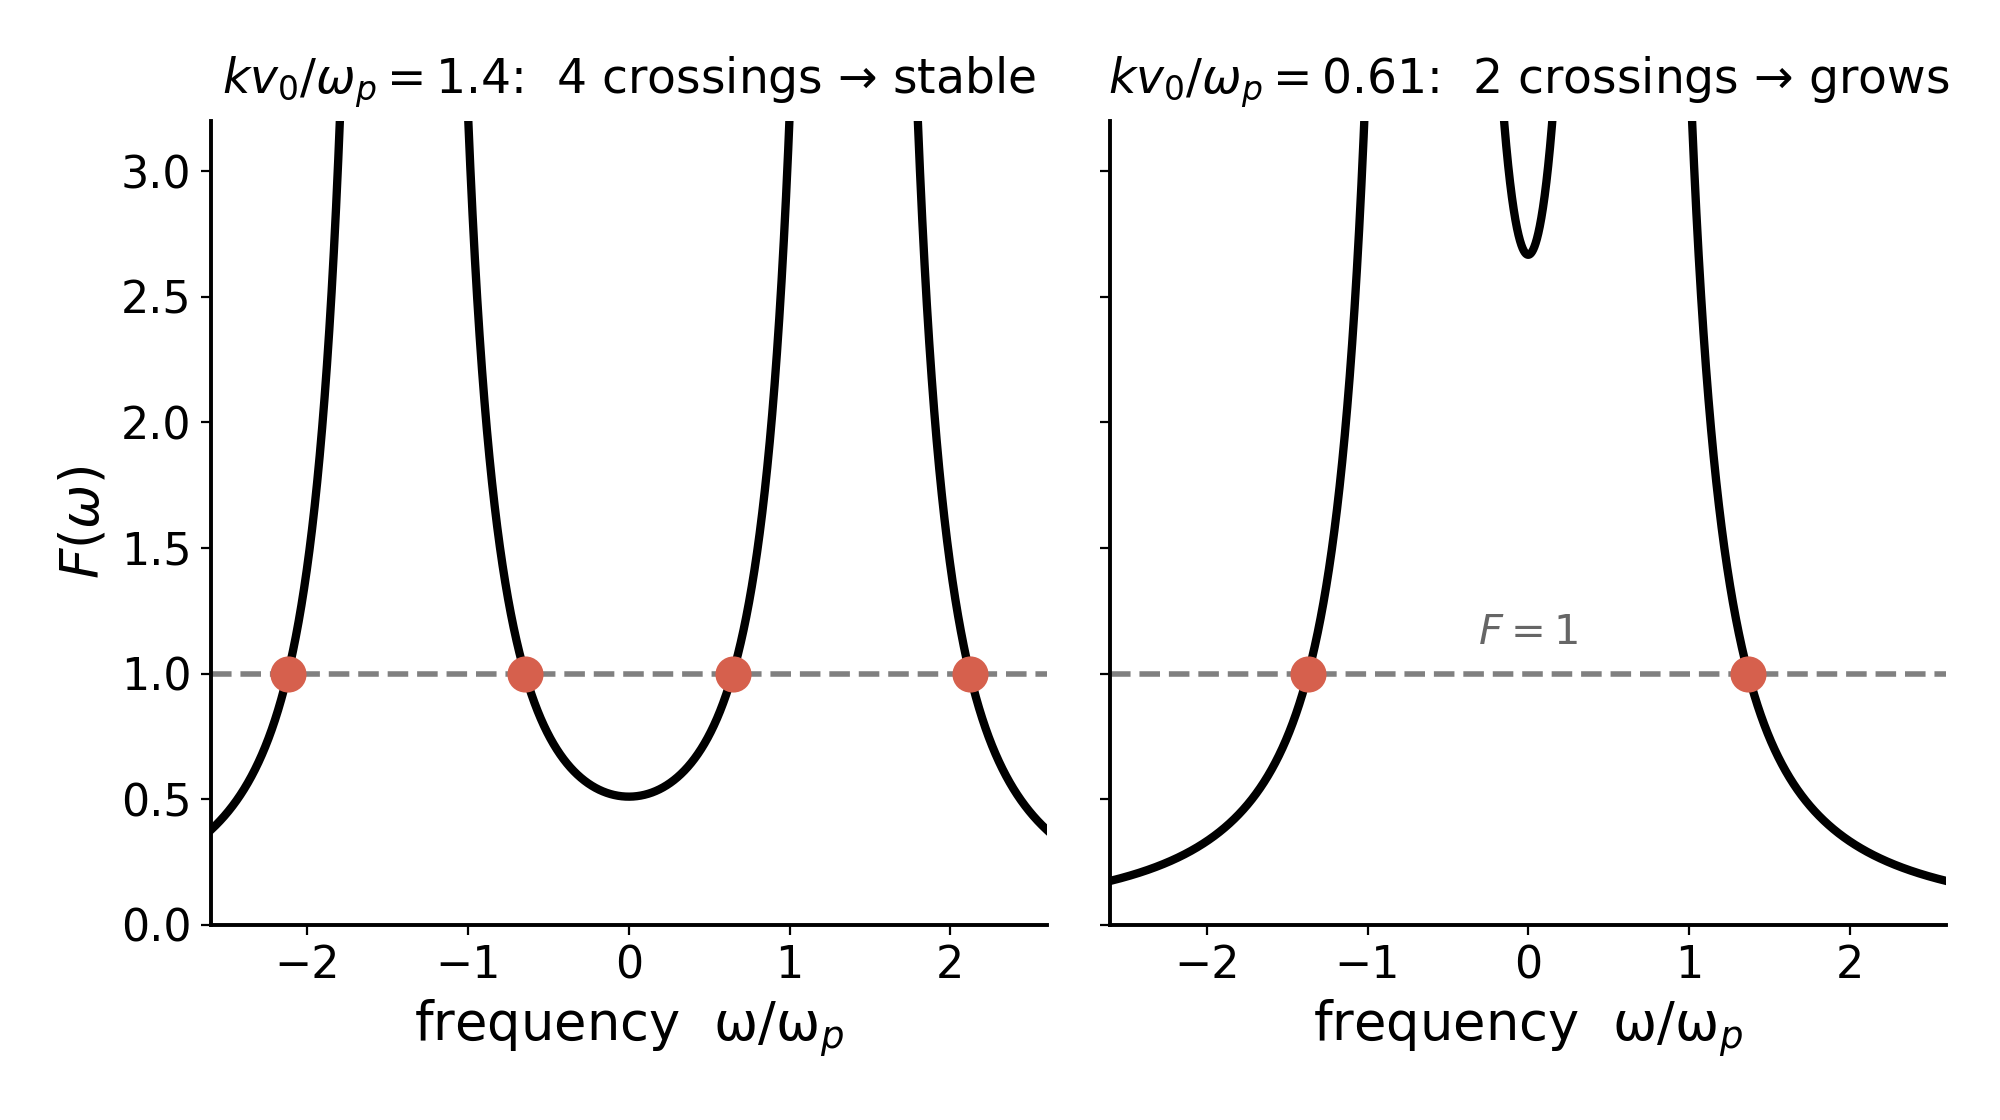
\includegraphics[width=\columnwidth]{figures/ee_dispersion_stable_unstable.png}
  \caption{Right-hand side of Eq.~\eqref{eq:disp} vs.\ $\omega$. Left: short wave, four
  crossings of 1, so four real roots and no growth. Right: longer wave, two crossings, so the
  other two roots are complex and the wave grows.}
  \label{fig:disp}
\end{figure}

% ===========================================================================
\section{How the simulation works}

A PIC code can't follow every electron, so it uses ``macroparticles'' that each stand for many
electrons (same charge-to-mass ratio, so they move the same way). The electric field is only
stored on a grid. Every time step the code (1) deposits the particles' current on the grid,
(2) updates the field, (3) interpolates the field back to each particle, and (4) pushes the
particles with Newton's law~\citep{BirdsallLangdon1991}. \textsc{Entity}~\citep{Entity} uses the
Boris pusher~\citep{Boris1970}, cloud-in-cell particle shapes, and a charge-conserving zigzag
current deposit~\citep{Umeda2003}. Nothing about the instability is put in by hand.

% ===========================================================================
\section{Setup}

The run is 1D and periodic. The beams move at $\pm0.1c$ (so $\vz\approx0.0995c$) and have a small
thermal spread, $v_{th}=0.01c$. The positive background is made of particles that never move.
Table~\ref{tab:params} lists the main numbers.

We used two runs that are the same except for how the particles start. In the \emph{random
start} the particles are placed randomly, which makes a lot of noise. In the \emph{quiet start}
they are evenly spaced, with each positive particle on top of an electron, so the starting charge
is basically zero (velocities are still random). The quiet run also has four times as many
particles. Together this makes the starting noise about 48 times smaller (28 times from the even
spacing and 1.8 times from the extra particles), so the wave gets about 4 more $e$-folds of clean
growth. All the figures below come from the quiet start; the random start is only used for
comparison.

\begin{table}[t]
  \centering
  \caption{Simulation parameters (code units, $c=1$). Particle counts are random start/quiet
  start.}
  \label{tab:params}
  \small
  \begin{tabular}{@{}ll@{}}
    \toprule
    Beam speed            & $\pm0.1c$ \\
    Thermal spread        & $v_{th}=0.01c$ \\
    Plasma frequency      & $\wpe\approx0.070$ \\
    Box length            & 100 ($\approx7\,c/\wpe$) \\
    Grid cells            & 12288 \\
    Cells per Debye length & $\approx17$ \\
    Particles per cell (each beam) & 4 / 16 \\
    Time step             & $\wpe\Delta t\approx3\times10^{-4}$ \\
    \bottomrule
  \end{tabular}
\end{table}

% ===========================================================================
\section{Results}

\paragraph{What the electrons do.}
Figure~\ref{fig:phase} shows the electrons in phase space (position vs.\ velocity). They start
as two flat beams. During growth the beams get wavy, and a few $1/\wpe$ after saturation they
have rolled up into vortices, which are electrons trapped in the wave.

\begin{figure}[t]
  \centering
  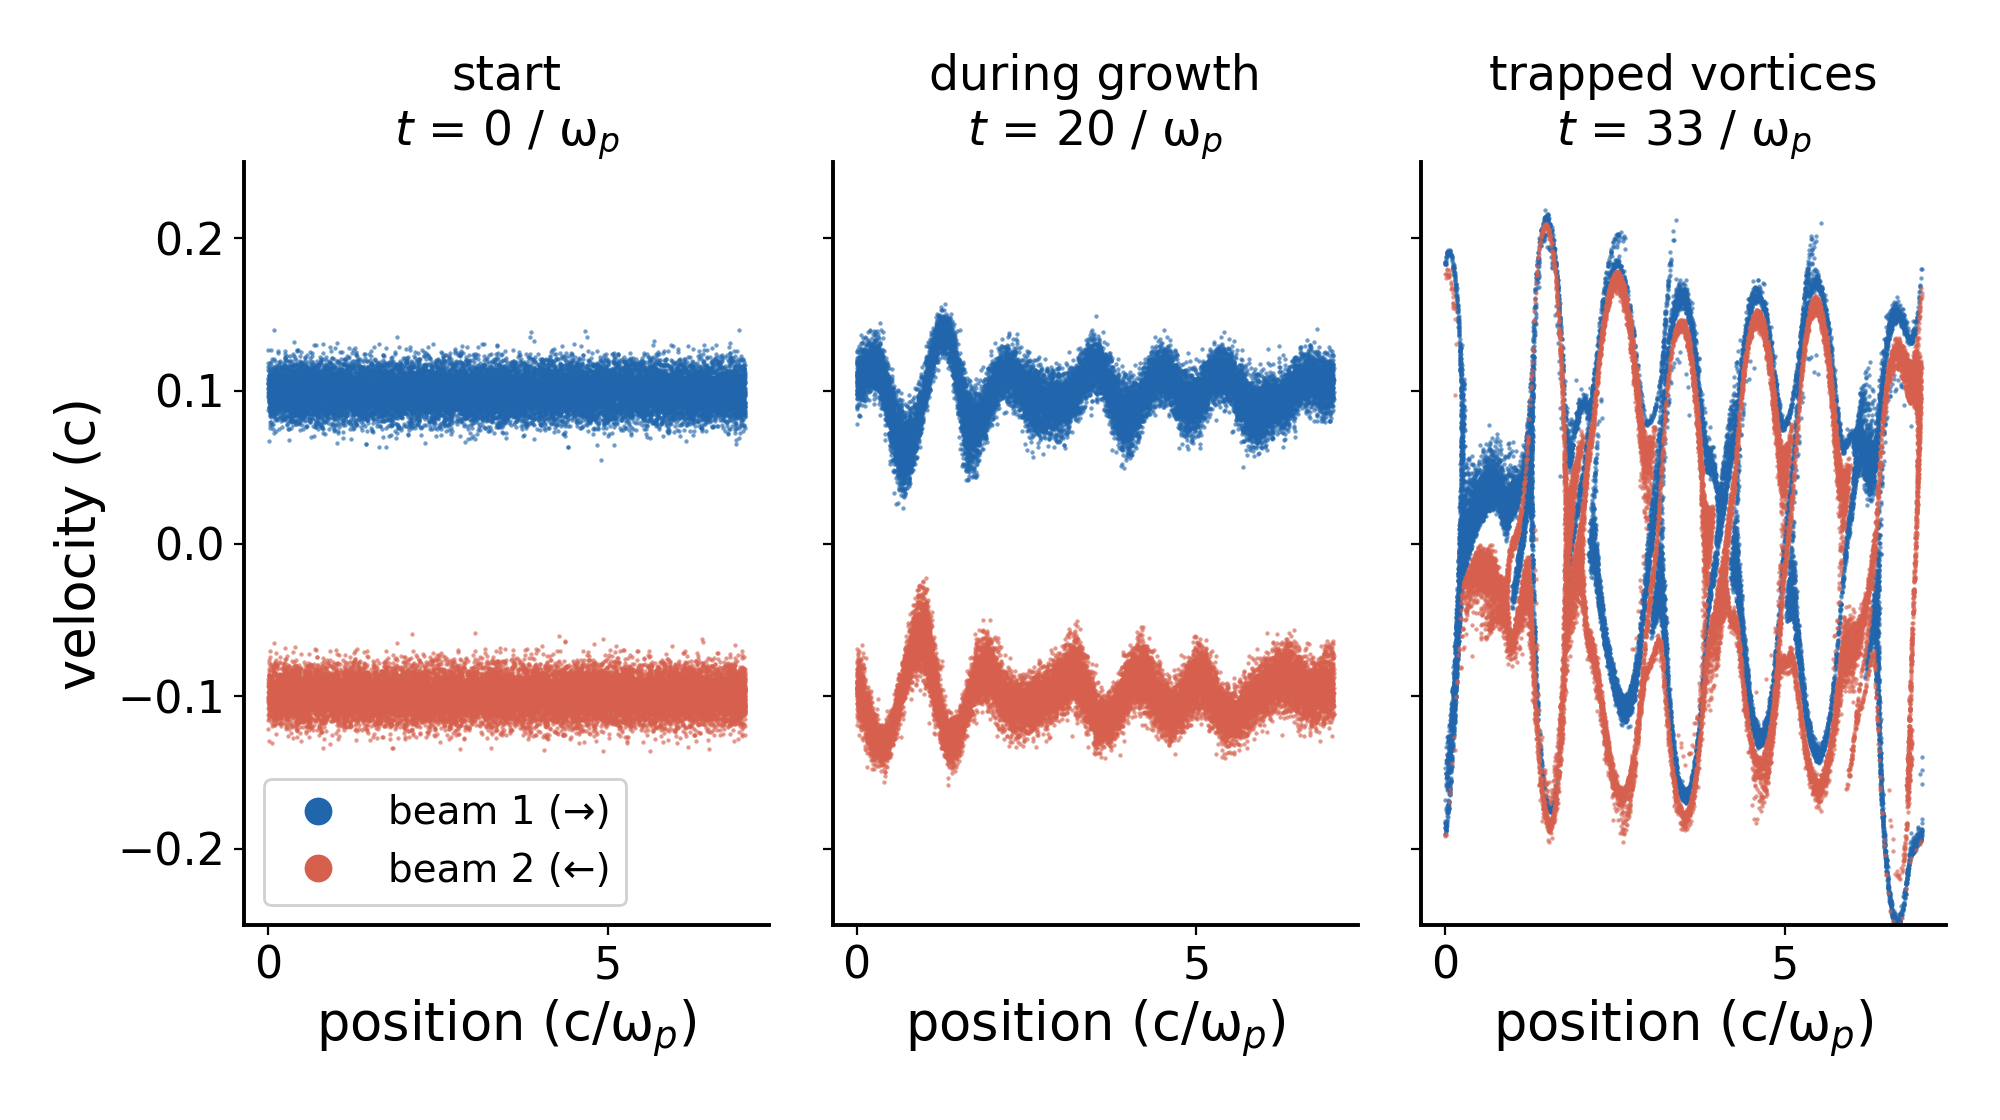
\includegraphics[width=\columnwidth]{figures/ee_phase_space.png}
  \caption{Phase space at $t=0$, 20 and $33/\wpe$: initial beams, linear growth, and trapped
  vortices about $6/\wpe$ after saturation.}
  \label{fig:phase}
\end{figure}

\paragraph{Exponential growth.}
To get the growth of each wave we Fourier transform $E_x(x)$ and follow each mode's amplitude
over time. Figure~\ref{fig:growth} shows the fastest one. The dashed line is the theory slope,
not fitted, just started at the same point. The simulation follows it for about 4.2 $e$-folds
(a factor of about 70) and then saturates at $t\approx27/\wpe$.

\begin{figure}[t]
  \centering
  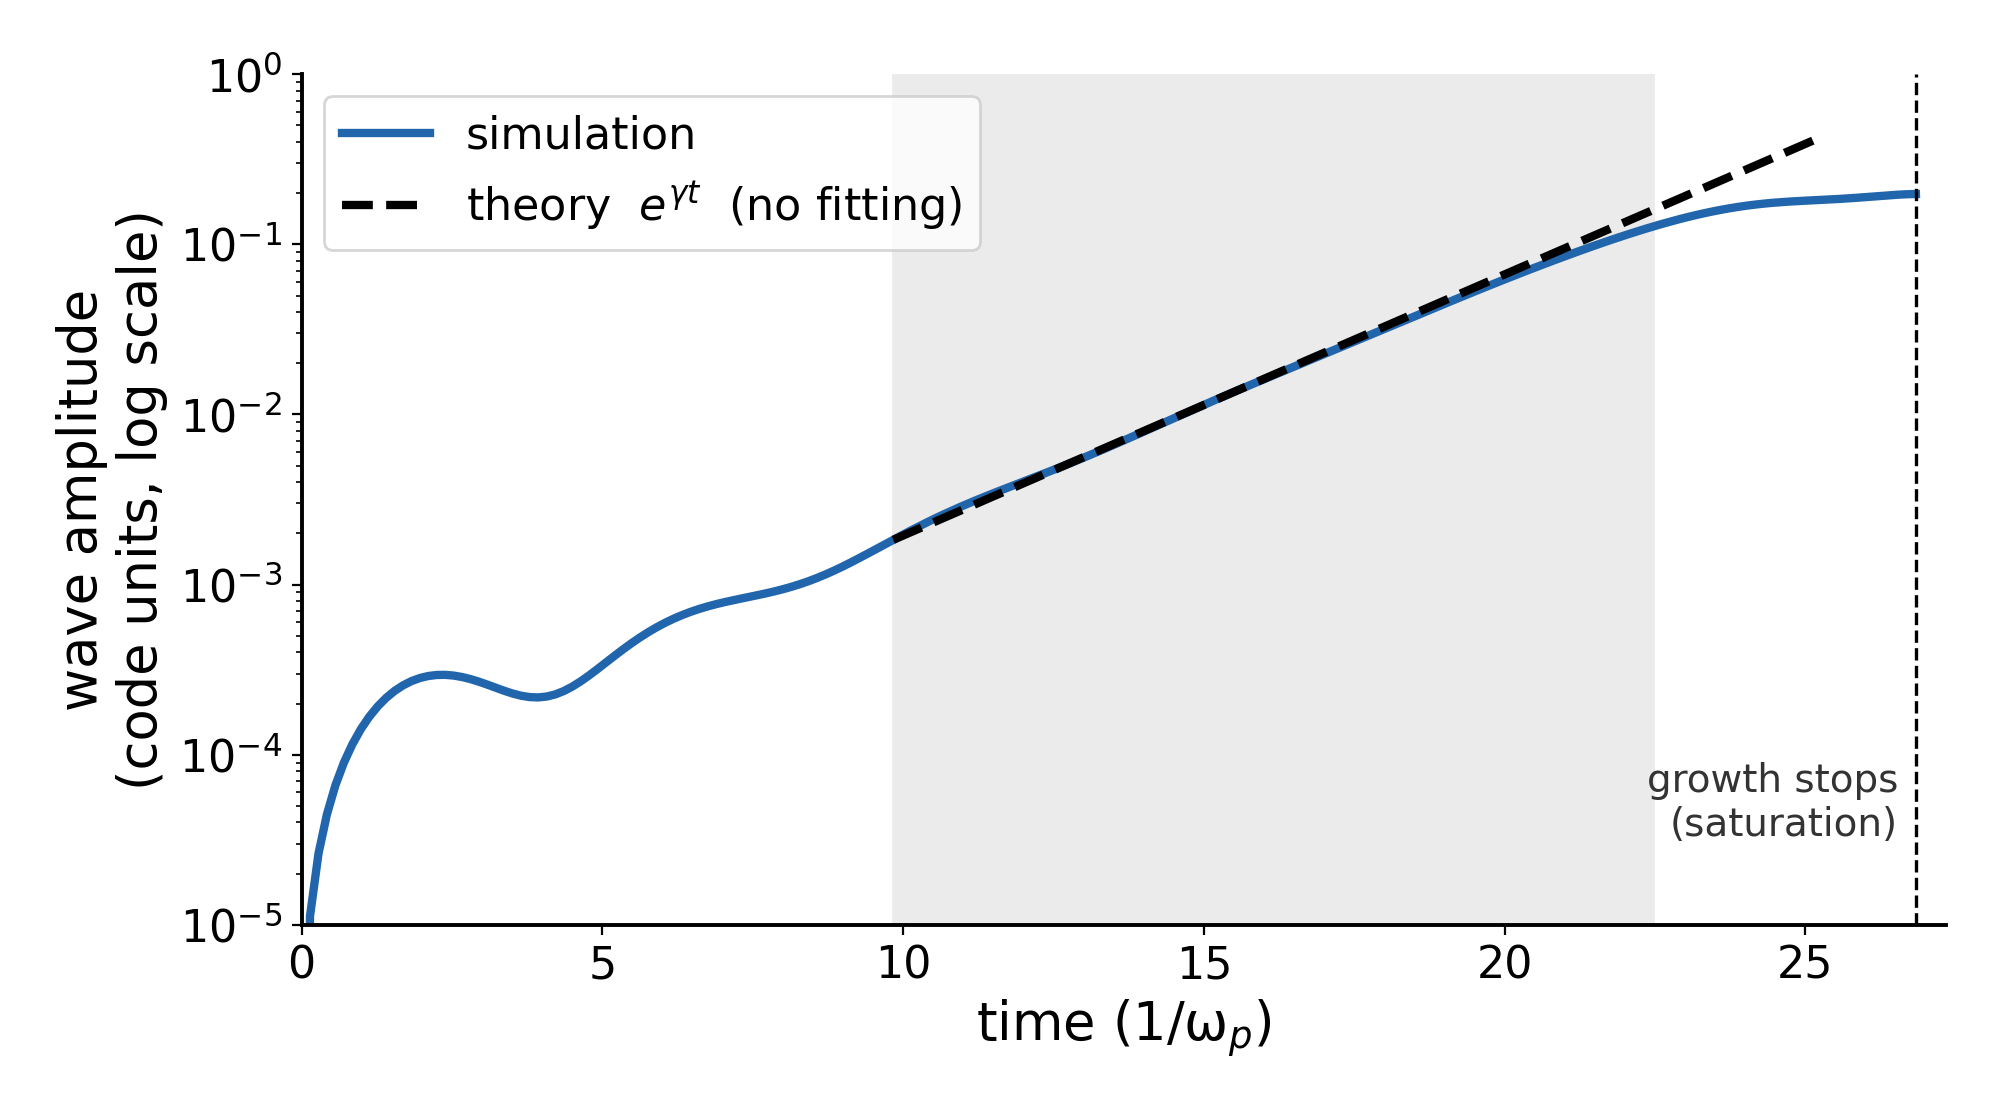
\includegraphics[width=\columnwidth]{figures/ee_growth_fastest_mode.png}
  \caption{Amplitude of the fastest-growing wave (quiet start) on a log scale. Dashed: theory
  $e^{\gamma t}$, not fitted. Shaded: the part used for fitting.}
  \label{fig:growth}
\end{figure}

\paragraph{The wave stays in place.}
Figure~\ref{fig:st} plots $E_x$ against position and time. The stripes are vertical, so the
wave is not moving, which is what $\mathrm{Re}\,\omega=0$ means. The measured real frequency is
at most $0.024\,\wpe$, basically zero.

\begin{figure}[t]
  \centering
  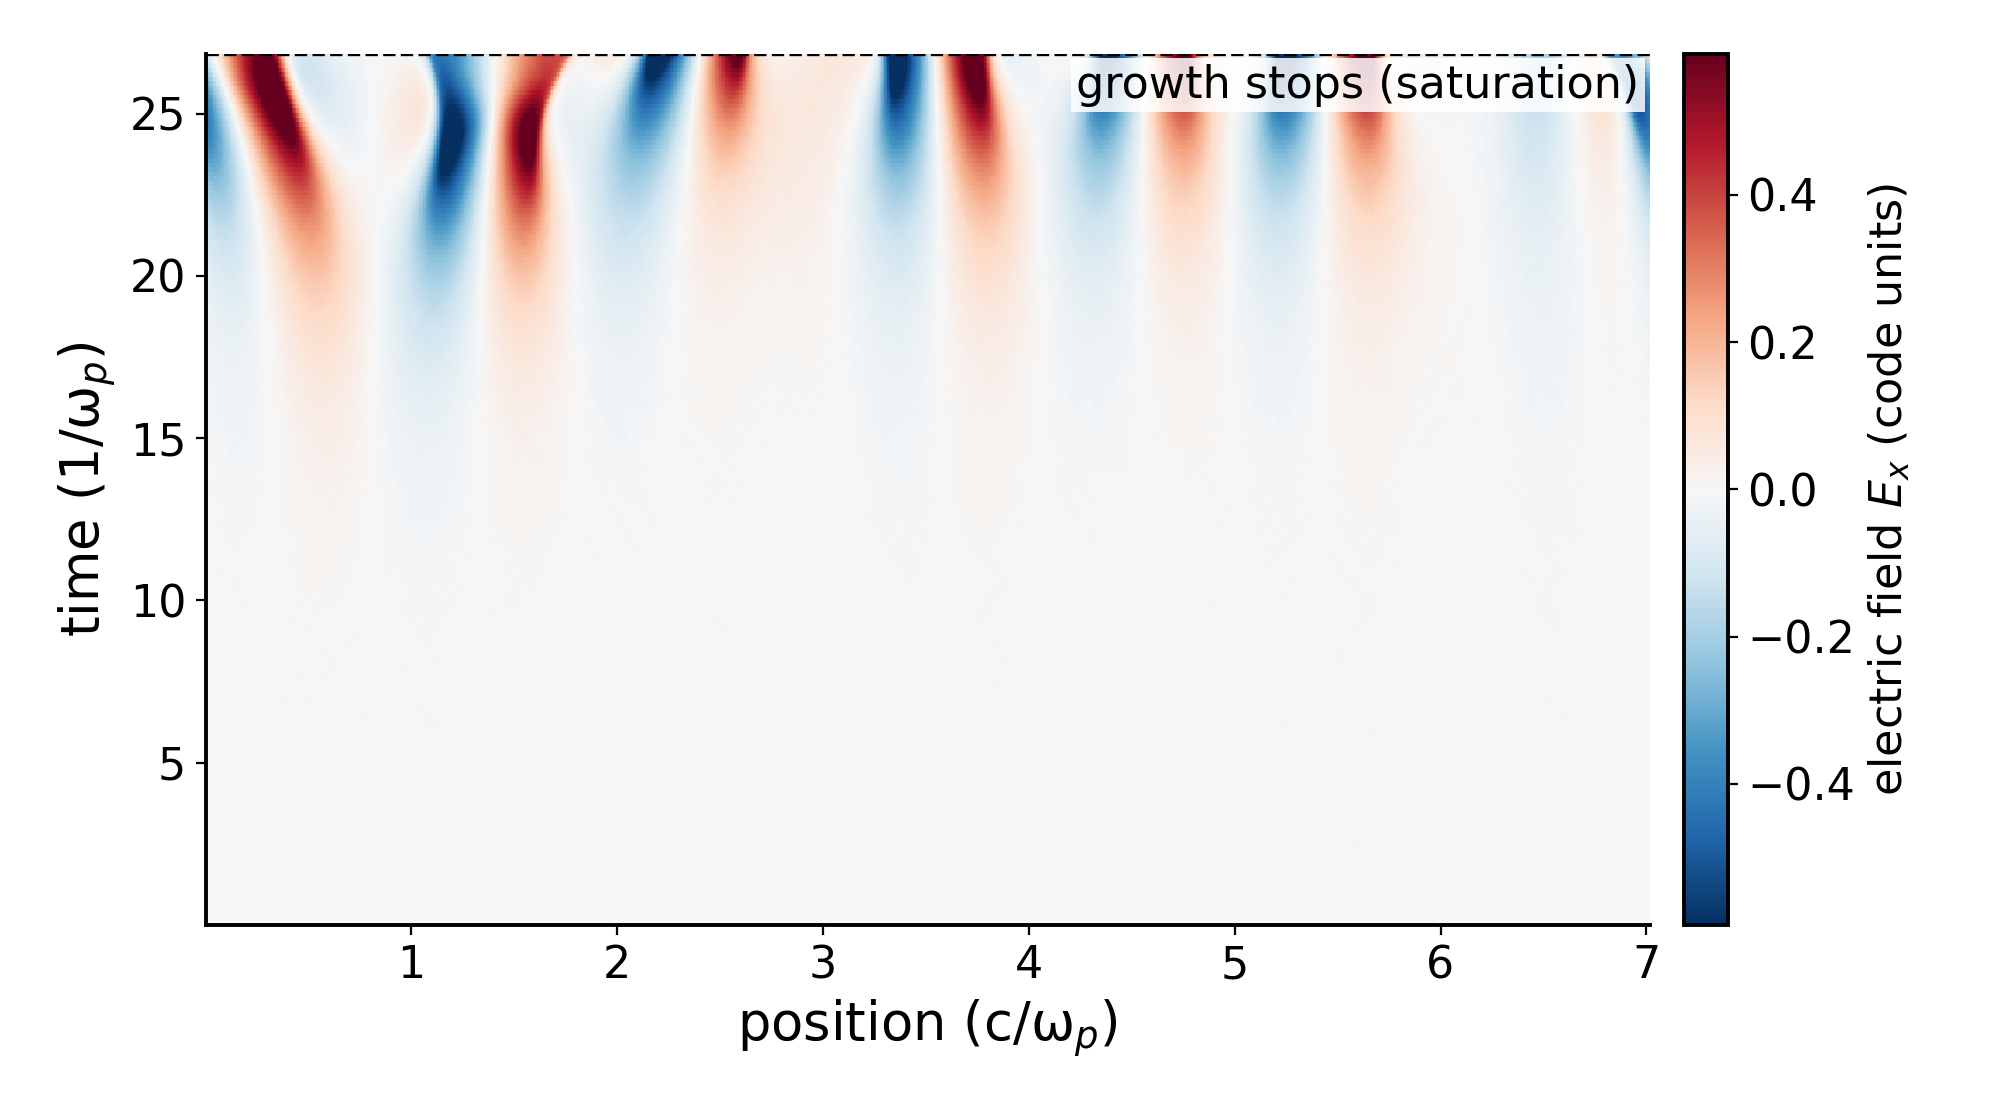
\includegraphics[width=\columnwidth]{figures/ee_spacetime_Ex.png}
  \caption{Electric field vs.\ position and time (quiet start). The stripes grow out of the noise
  and stay put until saturation (dashed line).}
  \label{fig:st}
\end{figure}

\paragraph{Growth rate vs.\ wavenumber.}
For each wave we fit straight lines to $\ln|E_k|$ over short windows across the growth phase and
take the median; the error bar is the spread between windows. Figure~\ref{fig:gammak} shows the
results on top of Eq.~\eqref{eq:gamma}. The fastest wave grows at $0.339\pm0.014\,\wpe$
compared with $0.354\,\wpe$ from theory. Seven waves land on the curve, and for the six in the
middle ($m=4$--$9$) the average of simulation over theory is $0.96\pm0.04$. The longest waves
($m=1$--$3$) and the one near the cutoff ($m=11$) grow too slowly to get above the noise, so we
can't measure them well. The simulation comes out about 4\% low; this is probably because our
beams are a little warm, which slows the growth a bit, but we didn't check that separately. For
comparison, the random start gave the same average but much more scatter
($0.99\pm0.16$), because the wave only had about 3 $e$-folds to grow.

\begin{figure}[t]
  \centering
  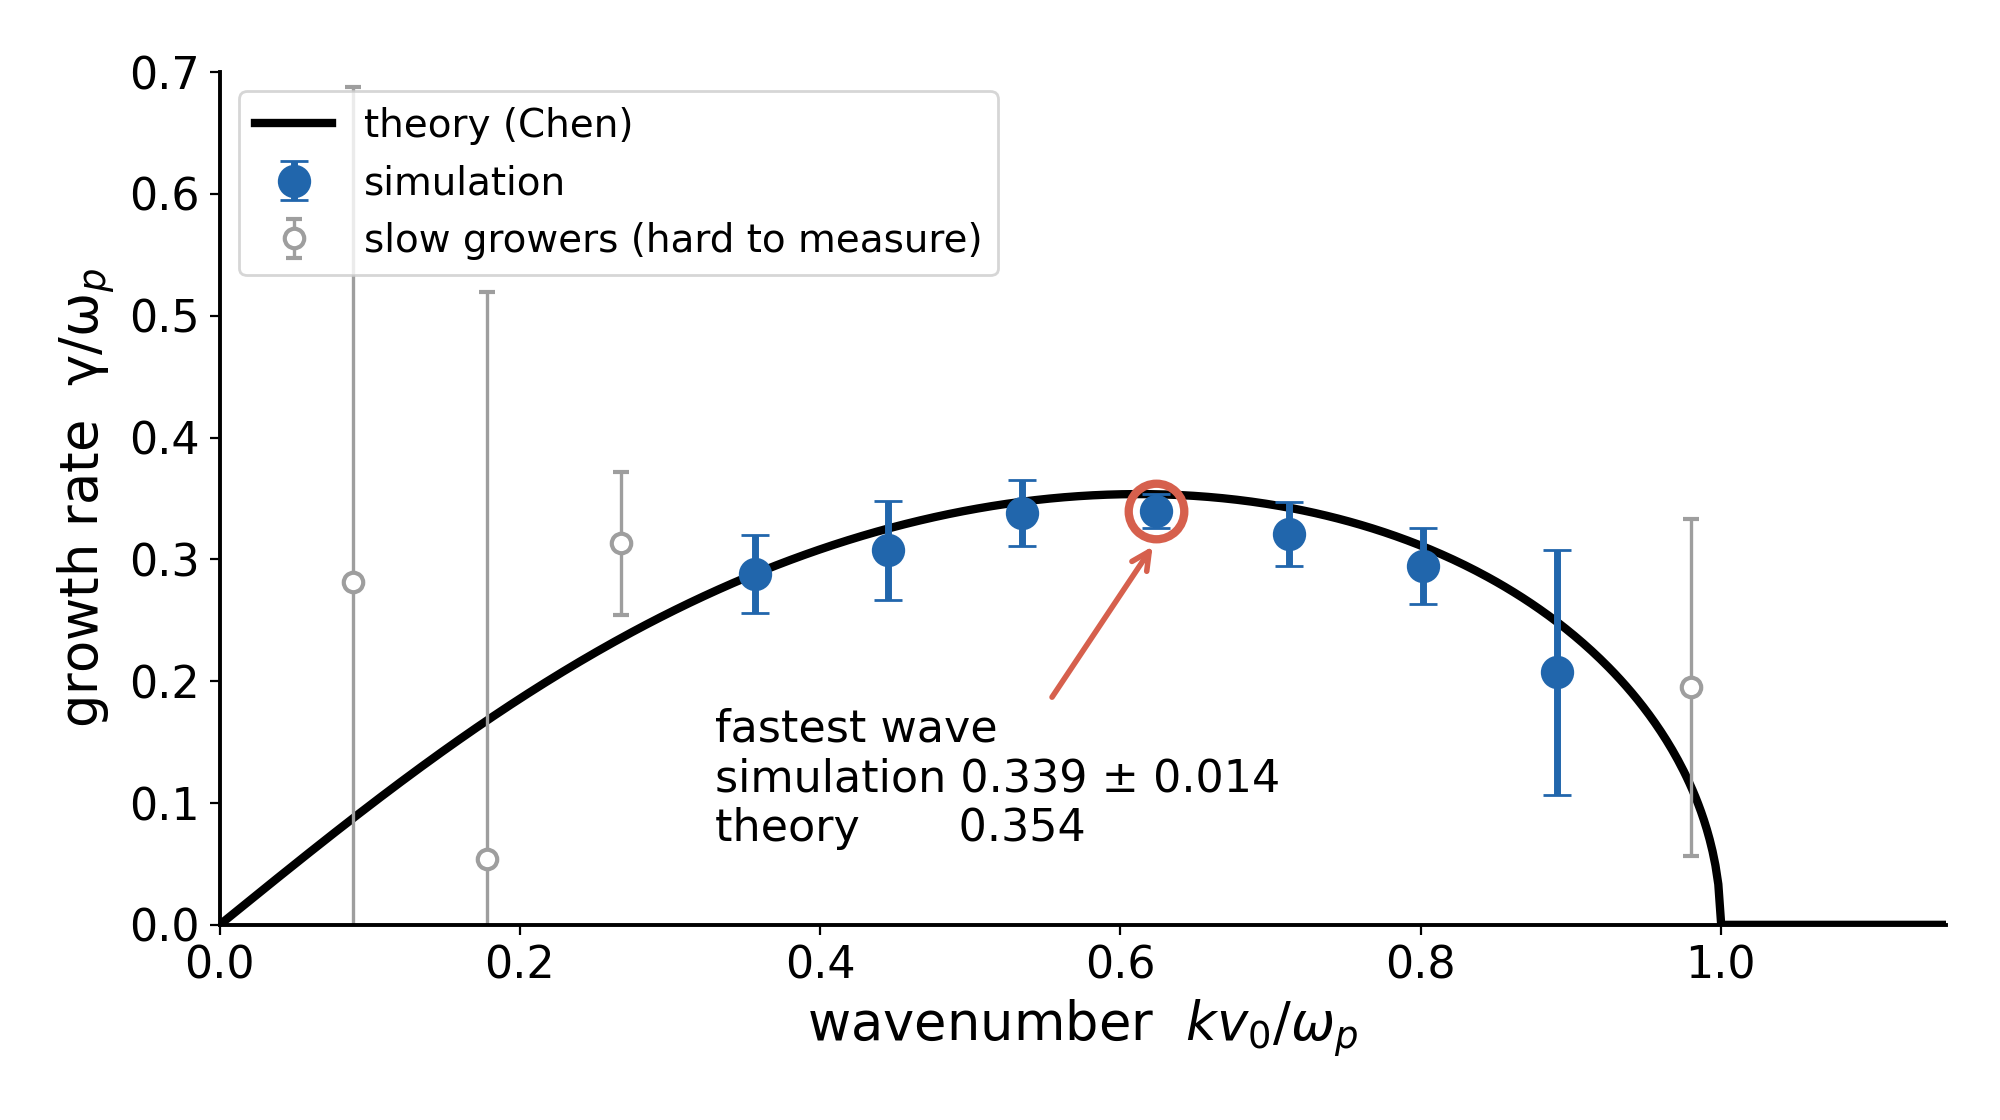
\includegraphics[width=\columnwidth]{figures/ee_growth_rate_vs_k.png}
  \caption{Measured growth rate of each wave (quiet start) vs.\ Chen's theory. Grey: slow growers
  that are hard to measure.}
  \label{fig:gammak}
\end{figure}

% ===========================================================================
\section{Conclusion}

The simulation shows what the theory predicts: a wave grows exponentially out of noise, it
doesn't move, and the growth rates follow Chen's curve. It is not perfect. The slowest waves are
hard to measure and the rates are about 4\% low, but the physics is clearly there. We also
learned that how the particles start matters a lot in PIC: evenly spacing them made the results
much cleaner.

{\small\setlength{\bibsep}{1pt}
\bibliographystyle{unsrtnat}
\bibliography{refs}}

\end{document}
